\section{Experimental Evaluation} \label{sec:experiment}

%\ls{It's unclear whether participants are creating products or product lines.}

In the previous case studies, we showed the viability of our software transplantation approach, implemented in \prodscalpel, to generate customized products from the existing codebase. Although the validation of the approach is based on empirical evidence, it  is  still important to test its efficiency by comparing it with other tools used to product line migration. Unfortunately, tool support for the reengineering process is limited, in general, they give support for specific activities, such as feature location, refactoring or quality assurance~\cite{Assuncao2017,Kruger2020}. To the best of our knowledge, there is currently no comparable tool that manages to automatically transplant features from distinct donor systems to generate a product line.
Therefore, we compare our approach with current state-of-the-art, namely human effort.
We conducted an experiment that reflects a real-world process of product line migration from existing codebases~\cite{Krueger2002}. In this section, we state our research objectives and describe in detail the experimental setting.\looseness=-1
 Our corpus and data collected are available at  the project webpage~\cite{ProjectWebpage}.
 
\subsection{Goal}
The goal of this experiment is to analyse the effectiveness and efficiency of our approach compared with the manual process of generating a product line from existing systems, performed by SPL  experts. In accordance with the guidelines for reporting software engineering experiments presented in ~\cite{Wohlin2012b}, we have framed our research objectives using the Goal Question Metric (GQM) method suggested by Basili~\cite{Basili1994}. Our goal is to:

\textbf{Analyse} a software transplantation approach to derive product variants 
\textbf{for the purpose of} comparison 
\textbf{with respect to} effectiveness and efficiency 
\textbf{from the point of view of} the researcher
\textbf{in the context of} an SPL project of product line migration from real-world systems.

\subsection{Research Questions}

In order to achieve the stated goal, we defined two quantitative research questions. These are related to the data collected during the period that the experiment was conducted. The questions are described as follows:

\begin{quote}
\textbf{RQ3.} \emph{How successful is \prodscalpel at feature migration when compared with human effort?}
\end{quote}
We would like to understand how well our approach automatically transfers all required code so that the target feature can run in an emergent product line and compare it with the manual process.

\begin{quote}
\textbf{RQ4.} \emph{How much feature migration time can be gained using \prodscalpel compared to the manual process?} 
\end{quote}
With this question, we evaluate the time spent by SPL experts to \emph{extract}, \emph{adapt} and \emph{merge} features to derive new product variants and compare these with the same processes when using \prodscalpel. 

\subsection{Measures}
With the objective to answer our research questions, we defined the measures that must be computed. For each question, one measure was defined. These are described as follows:

\textbf{M1.} For RQ3, the accuracy of our approach is computed by verifying if \prodscalpel successfully migrated new functionalities to a product line by passing all the regression, augmented regression and acceptance test suites. This will check whether or not the output of the transplanted feature is correct with respect to the given test suites. 

\textbf{M2.} For RQ4, we simply report the time that is spent on each activity to transfer the target features. These activities are: \emph{code extraction}, \emph{adaptation}, and \emph{merging}. The time for each of these activities was collected individually.

\subsection{Methodology}

We use two donor systems in our experiment:
\emph{NEATVI}\footnote{https://github.com/aligrudi/neatvi}, text editor extended from VI for editing bidirectional UTF-8 text and \emph{Mytar}\footnote{https://github.com/spektom/mytar}, an archive manager.  
Table~\ref{tab:instrumentation} gives more details about the systems used in this experiment. Having in mind manually inspecting a codebase to transfer a feature to a product line is hard, slow, and tedious~\cite{Mahmood2021}, we chose to select small systems to avoid participants getting tired. These codebases were available to download together with a script to automate setup of the environment.

\begin{table}[ht]
	\caption{Details of donors and product base systems used in our studdy.}
	\label{tab:instrumentation}
    \begin{center}
    	\begin{tabular}{l|lr|lr|lr} \hline
    		\multicolumn{1}{c}{Scenario} & \multicolumn{1}{|c}{Donors} & \multicolumn{1}{c|}{LoC}   & \multicolumn{1}{c}{Target features}       & \multicolumn{1}{c|}{LoC}  & \multicolumn{1}{c}{Host}& \multicolumn{1}{c}{LoC} \\\hline
    		I       & NEATVI & 5,276 & $\texttt{DIR\_INIT}$  & 239&\multirow{2}{*}{Product base}&\multirow{2}{*}{5,285} \\
    		II      & Mytar  & 1,046 & $\texttt{WRITE\_ARCHIVE}$ & 170&& \\\hline
    	\end{tabular}
    \end{center}
\end{table}

We recruited 20 SPL experts for the experiment that were divided into two different groups.  We chose to allow participants to use their own work environment by avoiding adaptation bias to a strange environment with the use of unknown tools.
Guidelines provided to the participants of \emph{Group A}\footnote{The guideline for perform the transplantation in  scenario I is available at \url{https://rb.gy/vydhbb}} and \emph{Group B}\footnote{The guideline for perform the transplantation in scenario II is available at \url{https://rb.gy/covz62}} consisted of a process description and systems documentation. Additionally, we provided training on reengineering software systems to SPL to ensure that all participants understood the experiment's objectives.

We used timesheets to record the effort spent on the necessary activities required to transfer features from an existing codebase to a product base, as previously mentioned. In addition to the timesheets, we used two forms to collect information about participants' experience. This data is shown in Table~\ref{tab:participants}. 
We also conducted a post-survey to better understand participants' problems encountered.  

\normalsize\subsection{Experimental design}

We answer our research questions by simulating a real reengineering process where two features must be transferred to a product line built over a product base. The experimental design was inspired by documented real product-line migration scenarios~\cite{Laguna2013, Assuncao2017}. 

In scenario I, we gathered a group of 10 SPL experts (called Group A) where each one of them had to manually re-transplant all portions of code that implement the feature $\texttt{dir\_init}$ to the product base. We removed this feature from the original version of \emph{NEATVI} to generate the product base used in this scenario. In scenario II, another group of 10 SPL experts (called Group B) tried to insert the feature $\texttt{write\_archive}$ from \emph{MYTAR} into the original version of NEATVI used as the product base. Here, we chose not to provide the post-operative product base used in the scenario I. Instead, we provide the original version of NEATVI, already with the feature $\texttt{dir\_init}$, to prevent possible code errors introduced in scenario I. As we analyse both scenarios separately, we believe that this strategy has minimized possible human bias.

The idea is to use each scenario to represent real scenarios of reengineering to SPL where system variants came from both similar (scenario I) and distinct codebases (an archive manager providing features to a text editor's product line - scenario II) as Figure~\ref{fig:experiment_design} shows.

\begin{figure}[t]
	\centering 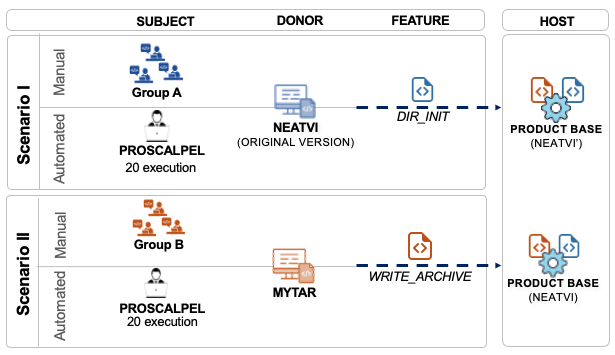
\includegraphics[width=0.8\textwidth]{images/experiment_design8.png}
	\centering 
	\caption{Experimental design: one factor with two treatments applied in two reengineering scenarios.}
	\label{fig:experiment_design}
\end{figure} 

In both scenarios participants are given the same inputs as \prodscalpel.
Thus the independent variable in our experiment is whether the feature migration process is automated or not.

In this experiment, the dependent variables are: success of the product line generation process and the payoff for using our approach. That is, to analyze the success of our approach (RQ3), we evaluate how often the transplanted features pass all the provided test cases.
To analyze the performance of the approach (RQ4), we measured the time spent by participants to extract, adapt and merge one feature into a product base in comparison with \prodscalpel's time to complete the same tasks.

\subsection{Pilot Study}

First, we conducted two pilot studies with 6 graduate students. 
We used the pilot study results to determine the amount of time needed to execute our tasks and the suitable size of features. This allowed us to estimate and plan the number of participants we needed for the main study. 
The pilot study also allowed us to assess whether the participants could properly understand the subject systems and the tasks they should perform. 

\subsection{Participants}

After the pilot study, we recruited 20 new participants: 2 undergrads (Un), 9 masters (M), 7 PhD. (PhD), and 2 Post-Ph.D. (Post-PhD). Most of them have more than 5 years of SPL experience and 10 years of software development. The participants are from ten different universities (from U1to U10) and the analysts/developers work in four different companies (C1, C2, C3, C4 and C5). To recruit them, we sent emails to professors from two universities, from different software reuse research groups, to suggest current and ex-members. 

Before the experiment, we asked them to answer an online survey, which we used to collect background data about their experience, mainly in software development and SPL\footnote{\url{https://rb.gy/ant4g8}}. 
We created balanced groups (A and B) of participants for each product line generation scenario, based on their experience. 
Table~\ref{tab:participants} shows the details of the participants involved in the experiment.

\begin{table}[t]
\centering 
	\caption{\textit{Details of participants' expertise (in years) and division into groups. Group A worked on scenario I, transplanting a feature from different versions of the same donor system as the host. Group B worked on scenario II,transplanting a feature from a donor system different to the host one}}
	\label{tab:participants}
	\resizebox{7cm}{!}{%
	\begin{tabular}{clllll} \hline
%	\toprule
		Group &Part. &Degree & Inst. & \multicolumn{2}{c}{Exp. (years)}\\ \cline{5-6}
		              &         &  &   & Dev.      &  SPL     \\\hline
		A       &P1  & MSc     & U7   & [1,5)     &  [5,10)  \\%magno
    	        &P2  & Un      & C5   & [10)      &  [1,5)   \\%mateus
		        &P3  & PhD     & U4   & [10)      &  [10)    \\%jonatas
		        &P4  & MSc     & U4   & [10)      &  [1,5)   \\%marco
		        &P5  & MSc     & U4   & [10)      &  [5,10)  \\%Djan
		        &P6  & MSc     & U4   & [10)      &  [5,10)  \\%Renata
		        &P7  & PhD     & U8   & [10)      &  [10)    \\%Alcemir
		        &P8  & PhD     & U9   & [10)      &  [1,5)   \\%Tiago
	            &P9  & PhD & U10  & [10)      &  [10)    \\%Larissa
	            &P10  & PhD     & U4   & [1,5)     &  [1,5)   \\\hline%Stefani
	            
		B       &P11   & MSc     & C1   & [10)      &  [1,5)   \\%Daniel
	            &P12   & MSc     & C2   & [1,5)     &  [1,5)   \\%Rose
		        &P13   & Un      & C3   & [10)      &  [1,5)   \\%Taijara
		        &P14   & PhD     & U1   & [10)      &  [10)    \\%Michele
		        &P15   & PhD     & U2   & [10)      &  [10)    \\%Paulo
		        &P16   & PhD     & U3   & [10)      &  [5,10)  \\%Tassio 
		        &P17   & MSc     & U4   & [5,10)    &  [5,10)  \\%Rafael X
		        &P18   & MSc     & C4   & [5,10)    &  [5,10)  \\%Anna
		        &P19   & PhD     & U5   & [10)      &  [10)    \\%Iuri
		        &P20  & MSc     & U6   & [5,10)    &  [1,5)   \\\hline%Loreno 
		        
	\end{tabular}
	}
\end{table}

\subsection{Operation} 

Before the participants receive their tasks, we introduced the experiment with a \emph{tutorial} on reengineering of existing systems into SPL. The tutorial took 30 minutes on average.

We provided the participants with the same input as the one required for \FOUNDRY, namely: feature entry points in the donor, the donor’s source code, and a prepared product base with the target insertion point.
We also supplied the participants with ice-box tests that could be used to guide the search for organ code modifications required to check if it continues to be executable when deployed in the host. Additionally, they received a few-sentence description of each feature in the target system and the system’s documentation with donor and host feature models. 

The direct costs of this experiment are related solely to the time spent by the researcher with the setup of the experiment itself. 
This involved: specifying the respective annotations for the entry point and insertion points of the features, which took approximately 13 minutes of work for scenario I and 17 minutes for scenario II; creating the test cases, necessary to validate the target features, taking approximately 16 minutes of programming activities; preparing the product base, which took approximately 14 minutes; then, approximately 34 minutes were spent creating all documentation of donor systems including the product base feature model.

To extend the emergent product line with a new feature transferred from the correspondent donor system, all participants were required to perform three activities based on the migration of system variants to the target product line~\cite{Krueger2001,Mahmood2021}: feature \emph{extraction}, \emph{adaptation} and \emph{merging}, with descriptions and instructions provided for each task.  

Initially, the participants had to identify and extract all code associated with the feature of interest to a temporary directory. 
Then, each participant had to adapt the extracted feature so it executes correctly in the product base environment, passing all unit tests. In practice, each participant had to change the feature source code to be compatible with the name space and context of its target insertion point in the product base. Finally, it had to insert the feature's code into the product base, and validate its correctness via regression testing.

\subsection{Data collection}

We have provided a task and time registration worksheet. While participants were conducting the assigned tasks, we asked them to take notes of which strategies were being used for each stage of the feature transfer process and why they are performing each specific task. It allowed us to capture strategies and performance data simultaneously. 

We have complemented the above setup with a post-survey. This way we can better understand participants' problems and differences between the manual and automated process in both scenarios. We have triangulated the data generated from the experiment with the responses we obtain from the pre and post-surveys.

To establish the time for feature transplantation using our automated approach, we ran \prodscalpel 20 times, and measure the average time spent on feature migration in each scenario. This average time was compared with the time spent by our participants on the manual reengineering process.

Based on our pilot study, we set a time limit of 4 hours for each manual and automated process. 
This is to allow for enough time to transfer required amount of LoC while avoiding participants getting bored or tired.

\subsection{Data Analysis}
\label{sec:experiment_data_analysis}
We used 22 pre-existing regression test suites designed by the \emph{NEATVI} developers to assess the success of \prodscalpel and manual transplantations and answer our \textbf{RQ3}. 
However, these were not designed to test \emph{NEATVI} as a product base with new variants and may not be sufficiently rigorous to find regression faults introduced by the reengineering process. 
To achieve better product line coverage, we manually augmented the host’s regression test suites with additional tests, our augmented regression suites.
Furthermore, we implemented an acceptance test suite for evaluating the transferred feature in both scenario I and II.
We have a total of 30 such tests in scenario I and 33 in scenario II. 
Our test suites provided statement coverage of 72.5\% to the post-operative product line in scenario I and 73.3\% to the post-operative product line in scenario II.

\subsection{Results and Discussion}
\label{sec:evaluation_results}

We summarise our results in Table~\ref{tab:transplantation_results}.  
We report the status of the product base and feature inserted by the participants, the time spent and the number of passing tests for the regression augmented regression and acceptance test suites \footnote{The time measured for the participants is available at \url{rb.gy/ant4g8}}. 
In the first scenario, only one of the participants was not able to finish the process before the timeout. On the other hand, half of the participants were able to finish the process before achieving the timeout in the second scenario and only three of them have been able to insert the target feature without breaking the product base. 

\begin{table}[t]
\centering 
    \caption{\textbf{Scenario I:} Donor: NEATVI - Product Base: NEATVI without the desired feature. \textit{Experiment results comparing the time of tool over 20 repetitions with the participants:column product line status shows the generated product line status by participants and tool; column \emph{Execution Time} shows the time spent on the feature transplant by the participants and the average time of 20 runs of \prodscalpel. We highlight the execution time of the participant that moqt quickly completed the task. Columns in \emph{Test Suites} show results for each test suite and report statement coverage (\%) for the postoperative host and for the organ. Columns marked with \emph{PASSED} report the number of passing tests.}}
	\label{tab:transplantation_results}
	\begin{tabular}{lcrrrr}\\\hline
		\multicolumn{1}{c}{}       & & & \multicolumn{3}{c}{Test Suites} \\            
		\cline{4-6}  
		 \multicolumn{1}{c}{Participants} & \multicolumn{1}{c}{ Product Line} & \multicolumn{1}{c}{Execution}& \multicolumn{1}{c}{Regre. (59\%)} & \multicolumn{1}{c}{Regre.++ (70.1\%)} & \multicolumn{1}{c}{Accept. (72.5\%)} \\
		\multicolumn{1}{c}{} & \multicolumn{1}{c}{Status} & \multicolumn{1}{c}{Time (minutes)} & \multicolumn{1}{c}{PASSED}  & \multicolumn{1}{c}{PASSED}  & \multicolumn{1}{c}{PASSED} \\\hline

		 P1 &\multicolumn{1}{c}{OK}  &\textbf{82}  & 22/22 &30/30 &3/3 \\
		     P2 &OK      &\textbf{88}  & 22/22  &30/30  &3/3\\
		    P3 &OK     &\textbf{77}  & 22/22 &30/30   &3/3\\
		     P4 &OK      &\cellcolor[gray]{.9}\textbf{68}  & 22/22  &30/30 &3/3\\
		     P5 &OK      &\textbf{81}  & 22/22  &30/30  &3/3\\
		     P6 &Broken & \multicolumn{1}{c}{\textbf{Timeout}} & 0/22     &0/30     &0/3 \\
		     P7 &OK      &\textbf{87}  & 22/22 &30/30   &3/3  \\
		     P8 &OK     &\textbf{83}  & 22/22 &30/30   &3/3 \\
		     P9 &OK      &\textbf{73}  & 22/22 &30/30  &3/3\\
		     P10 &OK     &\textbf{113} & 22/22  &30/30  &3/3\\
		 \hline 
		 \rowcolor[gray]{.9} \textbf{\prodscalpel} &\textbf{OK in 20/20 runs} &\textbf{20} &\textbf{22/22}   &\textbf{30/30}   &\textbf{3/3} \\
		 \hline
	\end{tabular}
    \bigskip
    \bigskip
    \bigskip
    \caption{\textbf{Scenario II:} Donor: Mytar - Product Base: NEATVI. All other columns are the same as in the previous table.}\label{tab:B}
	\begin{tabular}{lcrrrr}\\\hline
	\multicolumn{1}{c}{}       & & & \multicolumn{3}{c}{Test Suites} \\                       
		\cline{4-6}  
		\multicolumn{1}{c}{Participants} & \multicolumn{1}{c}{ Product Line} & \multicolumn{1}{c}{Execution}& \multicolumn{1}{c}{Regre. (70.1\%)} & \multicolumn{1}{c}{Regre.++ (71.9\%)} & \multicolumn{1}{c}{Accept. (73.3\%)} \\
		\multicolumn{1}{c}{} & \multicolumn{1}{c}{Status} & \multicolumn{1}{c}{Time (minutes)} & \multicolumn{1}{c}{PASSED}  & \multicolumn{1}{c}{PASSED}  & \multicolumn{1}{c}{PASSED}  \\\hline
		 P11 &Broken & \multicolumn{1}{c}{\textbf{Timeout}} & 0/22 & 0/33 & 0/2\\
		 P12 &Broken  & \multicolumn{1}{c}{\textbf{Timeout}} & 0/22 & 0/33 & 0/2\\
		 P13 &Error    &\textbf{181} & 0/22 & 0/33 & 0/2\\
		 P14  &Broken &\multicolumn{1}{c}{\textbf{Timeout}} & 0/22 & 0/33 & 0/2\\
		 P15 &Broken  &\multicolumn{1}{c}{\textbf{Timeout}}  & 0/22 & 0/33 & 0/2\\
		 P16 &Error    &\textbf{114} & 0/52 & 0/33 & 0/2\\
		 P17 &OK       &\cellcolor[gray]{.9}\textbf{104} & 22/22 & 33/33 & 2/2\\
		 P18 &OK       &\textbf{194} & 22/22 & 33/33 & 2/2\\
		 P19 &OK       &\textbf{131} & 22/22 & 33/33 & 2/2\\
		 P20 &Broken & \multicolumn{1}{c}{\textbf{Timeout}} & 0/22 & 0/33 & 0/2\\
		 \hline 
		 \rowcolor[gray]{.9} \textbf{\prodscalpel} &\textbf{OK in 19/20 runs} &\textbf{27} & \textbf{22/22} &\textbf{33/33}  &\textbf{2/2} \\\hline
	\end{tabular}
%}
\end{table}

For each scenario, we also report the number of \prodscalpel runs in which the product derived passed all test cases. For each scenario, we repeat each run 20 times. The success rate was retained for both scenarios I and II, where only one run timed out and the product line generated passed all tests from all test suites.

The results show success rate was retained in both scenario I and II, where we lost only one successful run in the timeout and all products derived passed all tests from all test suites.  
With regards to the manual process, nine participants have successfully transplanted the target feature in scenario I. 
In scenario II, seven of ten participants broke the product base when trying to transplant the target feature, while half of the participants were not able to transplant the feature within the timeout.

\begin{framed}
\noindent \textbf{RQ3:} Our results show that \prodscalpel outperformed participants in both scenarios with only one run timing out.  
Eight of twenty participants (considering both scenarios) were not able to transplant the target features without breaking tests.
\end{framed}

As stated in the definition of measure \textbf{M2} and to answer \textbf{RQ4}, we evaluate the payoff of \prodscalpel. Figure~\ref{fig:experiment_result_time_II} graphically shows the time spent on each activity performed in the reengineering to SPL process. In summary, Group A transferred the target feature from \emph{NETVI} to the product base in 1h24 minutes on average. \prodscalpel turned out to be quicker, successfully transplanting this feature in all 20 trials, taking an average of 20 minutes.

\begin{figure}[t]
	\centering 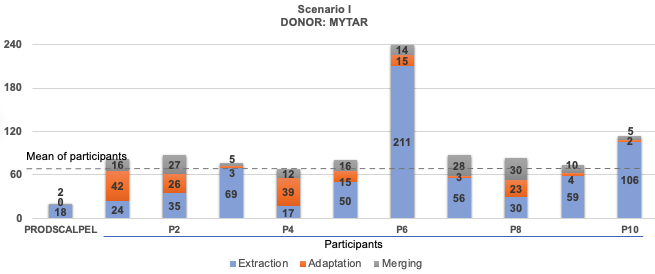
\includegraphics[width=0.9\textwidth]{images/experiment_result-SC1-4.png}
	\label{fig:experiment_result_time_I}
\end{figure} 
\begin{figure}[t]
	\centering 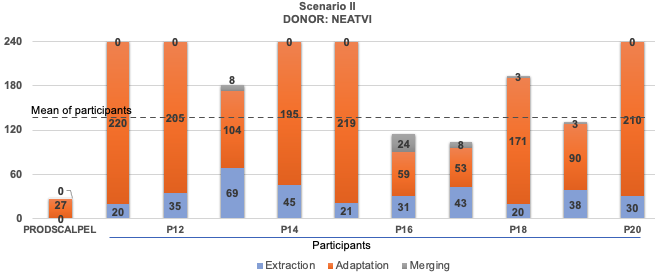
\includegraphics[width=0.9\textwidth]{images/experiment_result-SC2-4.png}
	\centering \caption{Time (in minutes) spent by participants and \prodscalpel on performing the three stages of SPL reengineering: feature \emph{extraction}, \emph{adaption} and \emph{merging}. The graph highlights the average time spent by participants who successfully generated new products.} 
	\label{fig:experiment_result_time_II}
\end{figure} 

Most of the participants from Group B had not completed the feature migration process from \emph{Mytar}  within the 4 hours time limit. Considering the participants that were able to finish the process (i.e., participants \emph{P17}, \emph{P18} and \emph{P19}) successfully (all tests passed) they spent an average of 2h23 minutes while \prodscalpel was able to complete this task in 19 of 20 trials in the timeout, taking 27 minutes on average.

By considering the time spent in both scenarios, the tool accomplished the product line generation process 4.8 times faster than the mean time taken by participants who were able to finish the experiment within the timeout.

\textbf{Statistical analysis of performance.} 
To establish statistical significance of our results we first establish statistical distribution of runtimes for each scenario through the Shapiro-Wilk~\cite{SHAPIRO1965} test. 
Next, we use ANOVA~\cite{Gelman2005} and Pairwise Student’s t-test analysis to test the hypothesis that \prodscalpel's runtimes are statistically lower when compared with the times required by the participants to complete the same task (p-value $<$ 2e-16). We rejected the null hypothesis for all pairs. Figure~\ref{fig:experiment_result_boxplot} graphically shows the time results for our two groups in comparison with \prodscalpel's performance. In scenario I, the preliminary information provided by the box plots indicates that all samples are normally distributed (W = 0.70445, p-value = 3.129e-05).

In scenario II, the normality test result showed a normal distribution with a W = 0.69378, p-value = 1.715e-06. Thus, we used ANOVA to hypothesis testing and Pairwise t-Student. Based on the ANOVA test and Pairwise t-Student, we rejected the null hypothesis (p-value $<$ 2e-16) that the distribution of the population is homogeneous.

We can conclude that \prodscalpel reduces developer effort to transfer features to a product line in both scenarios. For both simulation scenarios, there is a significant effect size between the tasks performed in a manual way and using \prodscalpel. 
Our participants had similar performance times in scenario I, with the exception of participant \emph{P6}. On the other hand, most of the participants of scenario II do not terminate the experiment before the 4-hour timeout. This last one is qualitatively explained by the participants in the post-survey where they mentioned it is hard to adapt a feature from one codebase to run in a different codebase. 
 
\begin{figure}[t]
	\centering 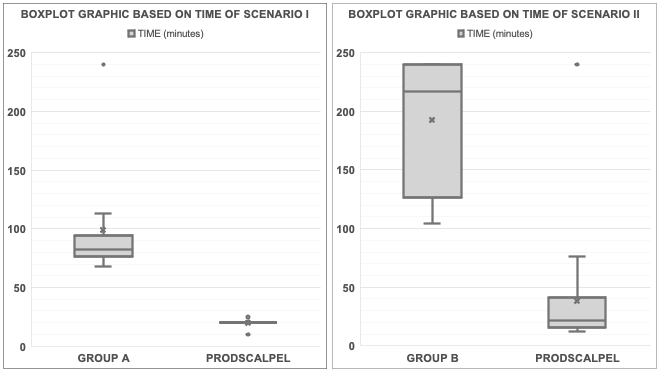
\includegraphics[width=0.9\textwidth]{images/experiment_time_results.png}
	\centering 
	\caption{Time results grouping automated and manual in both scenarios.  Scenario I: \emph{NEATVI} - Product Base; Scenario II: \emph{Mytar} - Product base.}
	\label{fig:experiment_result_boxplot}
\end{figure} 

\begin{framed}
\noindent \textbf{RQ4} The results confirmed that \prodscalpel outperformed participants transplanting two features 4.8 times faster, on average, compared to participants who finished the process within timeout.
\end{framed}

\section{Threats to Validity}

In this section we present threats to validity of our studies.

\textbf{External Validity.} The relatively small number and diversity of systems used for derive new products pose an external threat to validity. For our user study we applied our results to small programs due to the boundaries of an in-lab study; our results may not generalize to larger programs in the wild. We tried to mitigate it by constructing possible real-world scenarios, i.e., reuse of features from unrelated codebases and variations of the same real-world systems. Additionally, given that our approach was helpful even for small programs, we argue that it is likely helpful for larger systems as it is nearly impossible to incorporate new variants to a product line without a large understanding of the donor systems specifications~\cite{Assuncao2017} and without considerable adaption effort.

\textbf{Internal Validity.} Due to time expensive nature of a human study, we had only 20 participants. We tried to mitigate this issue by selecting participants with considerable experience in SPL projects. The other threat to the validity is the system size; small features are used in this experiment. We assume that inspecting the code to transfer a feature to a product line is hard, which has been confirmed in our post-study survey. We conducted a pilot study to mitigate threats arising from such issues.
Even with a limited execution time, we were able to transplant features from donors of significant size, considering the number of code lines of the subject systems, as shown in Table~\ref{tab:instrumentation}. 
Most participants were also able to complete the given tasks within the time limit.
We also use testing as means of validating our approach, which cannot provide a formal proof of correctness.  We used extensive testing to mitigate this risk. Moreover, testing is a standard approach to code evaluation in real-world scenarios due to its high scalability.
